\documentclass[11pt]{article}

\usepackage{geometry}
\geometry{a4paper, margin=2.3cm}

\usepackage{fontspec}
\usepackage{amsmath}
\usepackage{unicode-math}
% Fonts: Latin Modern (fontspec / unicode-math defaults) — reliably bundled with tectonic.

\usepackage{polyglossia}
\setdefaultlanguage{french}

\usepackage{microtype}
\usepackage{booktabs}
\usepackage{graphicx}
\graphicspath{{./}}
\usepackage{caption}
\captionsetup{font=small, labelfont=bf}
\usepackage[dvipsnames]{xcolor}
\usepackage[colorlinks=true, linkcolor=RoyalBlue, urlcolor=RoyalBlue, citecolor=RoyalBlue]{hyperref}
\usepackage{enumitem}

\setlength{\parindent}{0pt}
\setlength{\parskip}{0.45em}
\setlist{leftmargin=1.4em}
\setlength{\emergencystretch}{3em}

\newcommand{\tp}{^{\top}}
\newcommand{\bc}{\mathbf{c}}
\newcommand{\bb}{\mathbf{b}}
\newcommand{\bG}{\mathbf{G}}
\newcommand{\bZ}{\mathbf{Z}}
\newcommand{\bA}{\mathbf{A}}
\newcommand{\bd}{\mathbf{d}}
\newcommand{\bu}{\mathbf{u}}

\title{\bfseries Sélection à contribution optimale exacte à l'échelle génomique :\\ un solveur « support-first », sans matrice, validé contre optiSel et AlphaMate sur panels de marqueurs réels}
\author{\textbf{Adel Kaleche}\\[2pt] \small\itshape Chercheur indépendant, France. \\ \small\itshape Version française ; le manuscrit de référence est en anglais.}
\date{}

\begin{document}
\maketitle

\begin{abstract}
\noindent
La sélection à contribution optimale (OCS) --- maximiser le gain génétique sous une borne sur la coancestrie de la génération suivante --- arbitre entre gain et perte de diversité dans les programmes de sélection. Son goulot d'étranglement est la matrice de parenté qu'elle contraint : à l'échelle génomique cette matrice est dense et $n\times n$, coûtant $O(n^2 m)$ à construire et $O(n^2)$ à stocker, de sorte que les outils établis --- exact (optiSel) et heuristique (AlphaMate) --- heurtent un mur mémoire quand le nombre de candidats croît. Nous présentons \textbf{support-first}, un solveur exact reposant sur deux faits de l'OCS : le vecteur de contributions optimal a un support restreint à un petit sous-ensemble de candidats, et à support fixé le sous-problème contraint en parenté admet une forme fermée. Support-first fait croître le support par génération de colonnes à coût réduit et résout chaque support fixé en forme fermée, sans solveur itératif interne --- ce qui donne deux résultats distincts. D'abord, \emph{recevant} la matrice de parenté, l'ensemble actif exploite la parcimonie du support de la solution et atteint l'optimum exact 2 à 482$\times$ plus vite que la résolution à point intérieur d'optiSel selon le point de fonctionnement (12 à 132$\times$ à $\Delta F=1\%$, le plancher FAO du taux de consanguinité), car il évalue les candidats en $O(n^2)$, indépendamment du nombre de marqueurs. Ensuite, les produits de parenté $\bG\bc$ sont formés sans matrice à partir de la matrice de génotypes $\bZ$, de sorte que le solveur ne forme jamais la $\bG$ dense : il résout une instance ($n=40000$, $m=1000$) dont la matrice dense (11,9~Gio) ne tient pas. Cet avantage mémoire est le régime $m<n$ pour un $\bZ$ dense ; stocker $\bZ$ à deux bits par génotype (le chemin packé du solveur, vérifié comme rendant l'optimum identique) décale le crossover à $m<32n$ et tient un panel à l'échelle nationale ($n=5\times10^5$, $m=5\times10^4$) dans $6{,}25$\,Go là où la $\bG$ dense demanderait deux téraoctets. Le produit sans matrice coûte $O(nm)$ par itération, c'est donc l'élément habilitant à grand $n$, non une accélération universelle. Sur des panels réels (blé CIMMYT, porc PIC à 52k SNP, souris en population hétérogène avec sexe réel), support-first atteint l'optimum exact sur la frontière de coancestrie, en accord à $10^{-8}$ près avec un solveur conique à point intérieur qui, lui, s'arrête juste en deçà ; les plafonds de contribution par candidat ($0\le\bc\le\bu$) sont gérés. Support-first rend l'OCS exacte et reproductible praticable à l'échelle des populations.
\end{abstract}

\section{Introduction}

L'amélioration génétique du bétail et des plantes doit tenir deux objectifs en tension : maximiser le mérite génétique de la génération suivante, et conserver la diversité génétique dont l'érosion entraîne la dépression de consanguinité et ferme la porte à la réponse future à la sélection. La sélection à contribution optimale (OCS ; Meuwissen 1997) explicite ce compromis. Étant donné la valeur génétique estimée de chaque candidat et la matrice de parenté entre candidats, l'OCS choisit les contributions génétiques proportionnelles $\bc$ qui maximisent le gain espéré $\bb\tp\bc$ sous une borne sur la coancestrie moyenne de la descendance, $\bc\tp\bG\bc\le k$, les contributions étant non négatives et de somme un --- et, dans tout schéma d'accouplement réel, réparties de sorte que pères et mères fournissent chacun la moitié. L'OCS est le cadre de fait pour gérer la diversité, tant en sélection commerciale qu'en programmes de conservation, et la matrice de parenté génomique (VanRaden 2008) a largement remplacé son prédécesseur fondé sur le pedigree comme $\bG$ qu'elle contraint.

Avec des données génomiques, il s'agit d'un programme quadratique convexe à contrainte quadratique, équivalent à un programme conique du second ordre, et deux coûts en viennent à dominer à mesure que le nombre de candidats croît. Le premier est la matrice de parenté elle-même : dense et $n\times n$, elle coûte $O(n^2)$ à stocker et $O(n^2 m)$ à construire à partir de $m$ marqueurs, et à des dizaines de milliers de candidats elle ne tient plus dans la mémoire d'une station de travail. Le second est la résolution conique. Or le vecteur de contributions optimal est presque toujours porté par une poignée d'individus --- une parcimonie qui, comme nous le montrons, reste bornée à mesure que $n$ croît à point de fonctionnement fixé --- et les solveurs généralistes n'exploitent ni cela ni la structure peu coûteuse de la contrainte de parenté.

Les outils en usage couvrent l'exact et l'heuristique, mais partagent un même schéma : assembler la matrice de parenté complète et confier le problème entier à un optimiseur générique portant sur tous les candidats. La méthode originale de Meuwissen (1997), et son successeur Gencont2 (Dagnachew \& Meuwissen 2016), itèrent les conditions lagrangiennes sur l'ensemble complet des candidats. Le paquet optiSel (Wellmann 2019), l'outil exact de référence, formule l'OCS comme un programme conique pour un solveur primal-dual à point intérieur. Les formulations semi-définies (Pong-Wong \& Woolliams 2007) et de récents solveurs ADMM/JuMP (Waldmann 2025) suivent la même voie, ce dernier formant explicitement la matrice dense $\bG$ et ne tronquant les petites contributions qu'a posteriori. AlphaMate (Gorjanc \& Hickey 2018) troque l'exactitude contre une heuristique à évolution différentielle qui alloue aussi les accouplements. La seule tentative d'exploiter une parcimonie, Yamashita, Mullin \& Safarina (2018), exploite la parcimonie de l'\emph{inverse du pedigree} $\bA^{-1}$ --- une propriété de la matrice de données --- au sein d'une résolution à point intérieur sur tous les candidats ; ce n'est ni la parcimonie de la \emph{solution}, ni une méthode sans matrice fondée sur les génotypes. Aucun de ces outils n'exploite les deux faits qui rendent l'OCS génomique peu coûteuse : que le support optimal est petit à un point de fonctionnement donné, et qu'à support fixé le sous-problème contraint en parenté admet une solution en forme fermée. Aucun n'évite de matérialiser $\bG$, qui devient la contrainte limitante --- en mémoire et en temps de construction --- précisément aux tailles de population où l'OCS importe.

Nous présentons \textbf{support-first} (« le support d'abord »), un solveur OCS exact bâti sur ces deux faits. Il maintient un petit support de travail, initialisé avec le meilleur candidat de chaque sexe et étendu par une règle d'ensemble actif fondée sur le coût réduit : les candidats sont évalués contre les multiplicateurs courants, le plus avantageux est introduit, ceux qui deviennent négatifs sont retirés, le tout vers une unique borne de coancestrie fixée $k$. Chaque sous-problème à support fixé --- maximiser une forme linéaire sur un ellipsoïde intersecté avec les contraintes affines de somme (et de sexe) --- est résolu en forme fermée, en éliminant les contraintes d'égalité et en se ramenant à une équation quadratique scalaire dans le multiplicateur actif, sans solveur itératif interne. Les produits de parenté $\bG\bc$ sont formés sans matrice à partir de la matrice de génotypes centrée $\bZ$ sous la forme $\varepsilon\bc + \bZ(\bZ\tp\bc)/s$, de sorte que le solveur ne construit ni ne stocke jamais la matrice dense $n\times n$ $\bG$.

Les ingrédients pris isolément sont classiques, et nous n'en revendiquons aucun. Les méthodes d'ensemble actif qui suivent un petit ensemble de travail d'actifs détenus descendent de l'algorithme de la ligne critique de Markowitz (1956) pour la sélection moyenne--variance long-only, dont l'OCS est l'analogue contraint en parenté ; la forme fermée pour un objectif linéaire sur un ellipsoïde intersecté avec des contraintes linéaires est un résultat de valeur propre contrainte / équation séculaire (Gander, Golub \& von Matt 1989) ; et le produit sans matrice $\bZ(\bZ\tp\bc)$ est standard en prédiction génomique (VanRaden 2008 ; Legarra \& Misztal 2008). Notre contribution est leur \textbf{synthèse, spécialisée à l'OCS génomique} : une génération de colonnes fondée sur le coût réduit qui fait croître un support restreint vers une \emph{unique} borne de coancestrie --- par opposition au balayage paramétrique de \emph{toute} la frontière efficace de l'algorithme de la ligne critique --- avec le produit de parenté évalué sans matrice, de sorte que le coût d'une résolution suit la taille du support et le nombre de marqueurs, plutôt que la matrice dense $n\times n$. Les méthodes OCS antérieures touchent à la parcimonie du support, mais par l'autre bout : la méthode de Meuwissen (1997) résout sur l'ensemble complet des candidats et \emph{élague} ceux dont la contribution devient négative --- un ensemble actif décroissant sur le système dense $n\times n$. La nôtre fait croître le support par le bas via une génération de colonnes à coût réduit et ne forme jamais ce système ; à notre connaissance aucune méthode OCS antérieure ne combine ainsi un ensemble actif croissant et sans matrice fondé sur les génotypes ; le bénéfice tient à la combinaison plutôt qu'à l'une quelconque de ses parties.

Nous l'évaluons sur trois panels de marqueurs réels : un panel de blé CIMMYT ($n=599$), un panel de porc PIC ($n=3534$, 52k SNP) et un panel de souris en population hétérogène ($n=1814$, avec sexe réel). Il atteint l'optimum exact sur chacun, en accord à $10^{-8}$ près avec l'optimum conique. À coancestrie réalisée appariée, il coïncide avec les méthodes à point intérieur ; là où celles-ci s'arrêtent juste à l'intérieur de la contrainte, il atteint la frontière, de sorte que son léger avantage y est le budget de diversité qu'elles laissent inemployé, et non un optimum différent.

Cela donne deux avantages distincts. \emph{Recevant} la matrice de parenté, l'ensemble actif de support-first atteint le même optimum qu'optiSel 2 à 482$\times$ plus vite selon le point de fonctionnement (12 à 132$\times$ à $\Delta F=1\%$), car il évalue les candidats en $O(n^2)$, indépendamment du nombre de marqueurs --- le gain algorithmique de l'exploitation de la parcimonie du support. Former $\bG$ sans matrice échange cela contre le fait de ne jamais stocker la matrice $n\times n$, au prix de $O(nm)$ par itération ; c'est ce qui permet au solveur de tourner à des tailles de population où $\bG$ ne peut être formée, et --- le coût par itération suivant alors le nombre de marqueurs --- c'est la voie la plus rapide seulement jusqu'à une densité de marqueurs modérée, pas sur les panels les plus denses. Face à un solveur conique généraliste (Clarabel), l'avantage croît avec $n$ --- ${\sim}714\times$ à $n=10000$ à $\Delta F=1\%$, et ${\sim}76000\times$ à borne lâche --- dans une comparaison Rust contre Rust exempte de tout biais de langage. Face à AlphaMate, une heuristique pour le problème distinct de l'allocation discrète des accouplements, l'optimum exact n'est pas moins bon, à coancestrie appariée, sur la relaxation continue commune aux deux méthodes.

L'élément habilitant, toutefois, est la mémoire, pas la vitesse. Parce que la résolution ne forme jamais la matrice $n\times n$, elle tourne là où les outils établis ne le peuvent pas : à point de fonctionnement fixé ($\Delta F=1~\%$) sur des populations structurées, le support se maintient autour de 90 et la résolution autour de 0,3~s quand $n$ croît de 1000 à 40000, tandis que la $\bG$ dense que les alternatives doivent matérialiser atteint 11,9~Gio --- une empreinte 40$\times$ plus grande que $\bZ$, au-delà de la mémoire vive d'un portable de 8--16~Go. À cette taille, la question n'est plus la vitesse des outils établis, mais s'ils s'exécutent seulement. Support-first rend la sélection à contribution optimale exacte et reproductible praticable à l'échelle des populations, sur un ordinateur portable.

\section{Méthodes}

\subsection{Sélection à contribution optimale}

Pour $n$ candidats à la sélection de valeurs génétiques estimées $\bb\in\mathbb{R}^n$ et de matrice de parenté génomique $\bG\in\mathbb{R}^{n\times n}$, la sélection à contribution optimale choisit les contributions génétiques proportionnelles $\bc$ qui résolvent
\[
  \text{maximiser } \bb\tp\bc \quad\text{sous}\quad \bA\bc=\bd,\ \ 0\le\bc\le\bu,\ \ \bc\tp\bG\bc\le k.
\]
Les contraintes affines $\bA\bc=\bd$ encodent le budget de contribution. Dans la forme simplexe, une seule ligne $\bA=\mathbf{1}\tp$, $\bd=1$, impose $\sum_i c_i = 1$. Dans la forme \emph{sexuée} --- la vraie OCS, puisque chaque accouplement tire un parent de chaque sexe --- $\bA$ est la matrice d'incidence de sexe $2\times n$ (ligne 1 l'indicatrice mâle, ligne 2 l'indicatrice femelle) et $\bd=(\tfrac12,\tfrac12)\tp$, imposant $\sum_{\text{mâles}} c_i = \sum_{\text{femelles}} c_i = \tfrac12$. Le plafond par candidat $\bu$ borne la contribution d'un individu donné --- un sélectionneur laisse rarement un seul parent dominer une génération --- et est inactif à $\bu=1$. La borne de parenté $\bc\tp\bG\bc\le k$ plafonne la coancestrie moyenne de la descendance. Nous indexons les points de fonctionnement par le nombre effectif de parents contributeurs $N_e=1/\sum_i c_i^2$, avec le taux de consanguinité $\Delta F\approx1/(2N_e)$ (Woolliams \& Bijma 2000), et choisissons la borne $k$ atteignant un $N_e$ cible par bissection --- une ligne « $\Delta F=1~\%$ » est donc la borne donnant $N_e=50$. Ce $N_e$ est une quantité génomique de variance de contribution, un proxy défendable mais non identique du $N_e$ démographique auquel réfère le plancher FAO ($N_e\ge50$). Nous prenons $\bG$ comme la matrice de parenté génomique de VanRaden, $\bG=\bZ\bZ\tp/s+\varepsilon\mathbf{I}$, où $\bZ$ est la matrice $n\times m$ des génotypes centrés par deux fois les fréquences alléliques, $s=2\sum_j p_j(1-p_j)$, et $\varepsilon$ une faible régularisation ridge assurant la définie-positivité (la même matrice régularisée que contraignent les références coniques, de sorte que tous les solveurs affrontent un problème identique). Le programme est un programme quadratique convexe à contrainte quadratique, équivalent à un programme conique du second ordre.

\subsection{Deux faits structurels}

Support-first repose sur deux propriétés de l'optimum $\bc^*$. Premièrement, à une borne de parenté active, $\bc^*$ a pour support un petit ensemble $S=\{i: 0<c^*_i<u_i\}$ de contributions \emph{libres}, et $S$ est empiriquement borné quand $n$ croît à point de fonctionnement fixé (Résultats). Deuxièmement, sur la face où les contraintes de borne inactives sont supprimées (candidats fixés à 0 ou à leur plafond $\bu$), le problème restreint à $S$ --- maximiser une forme linéaire sur un ellipsoïde intersecté avec les contraintes affines --- admet une solution en forme fermée. Toute la difficulté est donc d'identifier $S$ et de savoir quels candidats sont à leur plafond ; tout le reste est une petite résolution directe.

\subsection{Forme fermée sur un support fixé}

Fixons un support $S$ de taille $|S|$, et notons $\bG_S$, $\bb_S$, $\bA_S$ les restrictions à $S$ ($\bA_S$ est $q\times|S|$ avec $q=1$ ou 2 lignes d'égalité). À l'optimum du problème restreint, la contrainte de parenté est active, et les conditions de stationnarité s'écrivent
\[
  \bb_S = \bA_S\tp\mu + 2\lambda\,\bG_S\bc_S,\qquad \bA_S\bc_S=\bd,\qquad \bc_S\tp\bG_S\bc_S=k,
\]
avec multiplicateurs $\mu\in\mathbb{R}^q$ et $\lambda\ge0$. Résoudre la stationnarité pour $\bc_S$ donne $\bc_S=\tfrac{1}{2\lambda}\bG_S^{-1}(\bb_S-\bA_S\tp\mu)$. Imposer les contraintes affines élimine $\mu$ : avec la matrice $q\times q$ $\mathbf{P}=\bA_S\bG_S^{-1}\bA_S\tp$ et le vecteur $\mathbf{q}_v=\bA_S\bG_S^{-1}\bb_S$,
\[
  \mu=\mathbf{P}^{-1}(\mathbf{q}_v-2\lambda\bd),\qquad\text{d'où}\qquad \bc_S=\mathbf{g}/(2\lambda)+\mathbf{h},
\]
où $\mathbf{g}=\bG_S^{-1}(\bb_S-\bA_S\tp\mathbf{P}^{-1}\mathbf{q}_v)$ et $\mathbf{h}=\bG_S^{-1}\bA_S\tp\mathbf{P}^{-1}\bd$ vérifient $\bA_S\mathbf{g}=\mathbf{0}$ et $\bA_S\mathbf{h}=\bd$, de sorte que $\bA_S\bc_S=\bd$ pour tout $\lambda$. En substituant dans l'ellipsoïde actif $\bc_S\tp\bG_S\bc_S=k$ et en posant $\alpha=\mathbf{g}\tp\bG_S\mathbf{g}$, $\beta=\mathbf{g}\tp\bG_S\mathbf{h}$, $\gamma=\mathbf{h}\tp\bG_S\mathbf{h}$, on obtient une unique équation quadratique scalaire dans le multiplicateur :
\[
  4(\gamma-k)\,\lambda^2 + 4\beta\,\lambda + \alpha = 0.
\]
On prend la racine positive maximisant $\bb_S\tp\bc_S$. Comme $\bG_S\mathbf{g}=\bb_S-\bA_S\tp\mathbf{P}^{-1}\mathbf{q}_v$ et $\bG_S\mathbf{h}=\bA_S\tp\mathbf{P}^{-1}\bd$ sont déjà disponibles, $\alpha,\beta,\gamma$ ne coûtent que des produits scalaires --- pas de seconde factorisation. Une résolution restreinte est donc : une factorisation de Cholesky de $\bG_S$, des remontées pour les $q+1$ seconds membres $[\bA_S\tp\mid\bb_S]$, une inversion $q\times q$ ($q\le2$) et une équation quadratique scalaire --- sans itération interne. Le cas simplexe ($q=1$, $\bA_S=\mathbf{1}\tp$) est identique et se réduit à une équation quadratique scalaire en $\mu$. Quand les égalités déterminent entièrement $\bc_S$ ($|S|=q+1$), les contributions sont forcées --- $(\tfrac12,\tfrac12)$ dans le cas sexué --- et l'on pose $\lambda=0$ (le sous-cas actif est de mesure nulle, comme pour un support singleton). La résolution renvoie « infaisable sur $S$ » quand $S$ manque d'un sexe ou que l'ellipsoïde ne rencontre pas l'enveloppe affine, signal pour agrandir $S$.

\subsection{L'algorithme support-first}

Le support est trouvé par génération de colonnes en ensemble actif. Il est initialisé avec le meilleur candidat de chaque sexe, $S=\{\arg\max_{\text{mâles}} b,\ \arg\max_{\text{femelles}} b\}$. Chaque itération résout la forme fermée sur le $S$ courant et se ramifie :

\begin{itemize}
\item \textbf{Infaisable sur $S$} (le support est trop apparenté pour atteindre la borne $k$) : ajouter les candidats les moins apparentés, ceux de plus petit $(\bG\bc)_j$, par paquet doublant $|S|$. Cette phase de faisabilité, lorsqu'elle se faisait un candidat à la fois, était le coût dominant ; le traitement par paquets a réduit le nombre total d'itérations d'environ un facteur trente, pour un optimum identique.
\item \textbf{Une contribution est négative} : retirer tout $i$ tel que $c_{S,i}\le0$, en les marquant tabous à la réintroduction jusqu'à la prochaine amélioration véritable, puis re-résoudre ; si un retrait vide un sexe, son meilleur candidat est réintroduit.
\item \textbf{Sinon} : évaluer chaque candidat $j\notin S$ par son coût réduit $r_j=b_j-\mu_{\text{sexe}(j)}-2\lambda(\bG\bc)_j$, et ajouter le maximiseur si $r_j>\text{tol}$ ; si aucun n'est positif, arrêter. Un ajout véritable vide l'ensemble tabou.
\end{itemize}

Le problème étant convexe, un point réalisable où aucun candidat n'a de coût réduit positif satisfait les conditions de Karush--Kuhn--Tucker et constitue l'optimum global ; la correction n'est donc pas heuristique. L'ensemble tabou, conjugué à un seuil de dégénérescence calibré sur l'ordre de grandeur des coefficients, a empêché tout cyclage sur chaque instance résolue ici, sans que nous prouvions la terminaison finie en général. La forme fermée reste bien conditionnée en pratique : avec le ridge $\varepsilon$, $\kappa(\bG_S)$ va d'environ 10 à 4000 aux supports opérationnels sur les panels réels (le plus élevé sur les lignées de blé autogames), et un bloc de génotypes exactement dupliqués --- une $\bG_S$ singulière sans le ridge --- se résout tout de même en un optimum KKT réalisable, les doublons se partageant leur contribution à parts égales. L'évaluation par coût réduit vers une \emph{unique} borne fixée $k$ distingue la mise à jour du support de l'algorithme de la ligne critique, qui modifie l'ensemble actif de $\pm1$ le long d'un multiplicateur balayé pour tracer toute la frontière efficace.

Un plafond par candidat $\bc\le\bu$ est absorbé par le même ensemble actif sans perte de la forme fermée. Une contribution libre qui dépasse son plafond est fixée à $u_j$ et déplacée dans un ensemble \emph{supérieur} $U$ ; un candidat déjà dans $U$ est relâché vers l'ensemble libre quand son coût réduit devient négatif. À $U$ fixé, la résolution restreinte conserve sa structure --- les contributions fixées entrent dans le second membre affine sous la forme $\bd-\bA_U\bu_U$ et dans l'ellipsoïde actif comme un décalage sans matrice $\bG_{\cdot U}\bu_U$ plus une constante, laissant la même factorisation de Cholesky et la même équation quadratique scalaire. La résolution bornée se réduit à la résolution non bornée quand aucun plafond n'est actif, et atteint le même optimum qu'un solveur conique à point intérieur sur le programme conique $\bc\le\bu$ correspondant, sous plafonds actifs.

\subsection{Produits de parenté sans matrice}

Tout produit de parenté complet est formé sans matérialiser $\bG$ :
\[
  \bG\bc = \varepsilon\,\bc + \bZ(\bZ\tp\bc)/s,
\]
deux produits matrice--vecteur contre la matrice de génotypes $n\times m$, en $O(n\cdot m)$ en temps et $O(n\cdot m)$ en mémoire pour $\bZ$ contre $O(n^2)$ pour une $\bG$ dense. La $\bG_S$ restreinte n'est assemblée que sur le support. $\bZ$ est conservé à deux bits par génotype (les trois dosages n'en demandent pas plus), le centrage appliqué à la volée par des corrections rang-1, de sorte que son empreinte est $nm/4$ octets --- encore $32\times$ sous un $\bZ$ dense en $f64$ ; les résolutions packée et dense rendent le même optimum à la précision machine. C'est l'élément habilitant à grand $n$, où la matrice dense $n\times n$ $\bG$ est infaisable à stocker ou coûteuse ($O(n^2 m)$) à construire ; ce n'est pas une accélération de boucle interne quand $m>n$, et l'avantage sur les références coniques est algorithmique --- le petit ensemble actif --- indépendant de ce choix.

\subsection{Implémentation et reproductibilité}

Le solveur est implémenté en Rust sur une pile purement Rust : algèbre linéaire dense (la factorisation de Cholesky et les remontées sur le support) via \texttt{faer}, sans dépendance système BLAS/LAPACK, sans \texttt{unsafe}, et avec un générateur aléatoire reproductible amorcé pour les générateurs synthétiques. Un solveur conique à point intérieur (\texttt{clarabel}) n'est inclus que comme oracle indépendant de contre-vérification. La correction est attestée par des tests unitaires à certificat KKT sur une plage de bornes $k$ --- un résultat \texttt{Solved} est toujours réalisable, sur le budget et réparti par sexe --- et par un accord inter-langage : sur une instance active, le \texttt{solve\_sexed} en Rust reproduit un optimum de référence NumPy à une différence de gain de $1{,}5\times10^{-14}$ près. La compilation est conditionnée à \texttt{cargo fmt}, \texttt{cargo clippy -D warnings} et la suite de tests.

\subsection{Données et références de comparaison}

La méthode est évaluée sur trois panels de marqueurs publics : un panel de blé CIMMYT (\texttt{BGLR}, $n=599$), un panel de porc PIC ($n=3534$, 52k SNP, avec valeurs génétiques estimées réelles) et un panel de souris en population hétérogène (\texttt{BGLR}, $n=1814$, avec sexe enregistré, 934 mâles et 880 femelles, l'indice de masse corporelle servant de critère de sélection). Pour chacun, $\bG$ est la matrice de VanRaden avec régularisation ridge $\varepsilon=10^{-5}$.

Une quatrième instance est dérivée du panel PIC et est la seule à porter simultanément une vraie valeur génétique et un sexe réel. Les données PIC sont livrées avec un pedigree, et un pedigree assigne le sexe sans ambiguïté : un animal figurant en colonne père est mâle, en colonne mère femelle. Le croisement avec les animaux génotypés restitue un sexe enregistré pour 1194 des 3534 (390 pères, 804 mères, aucun n'apparaissant comme les deux), tous porteurs d'une valeur génétique estimée réelle issue de l'évaluation associée (précision moyenne 0,811 sur le caractère 3). Les fréquences alléliques, et donc $\bG$, sont recalculées sur les animaux retenus. Le sexe n'étant récupérable que pour les animaux devenus parents, ce sous-panel est un sous-ensemble post-sélection plutôt qu'un échantillon aléatoire de candidats --- une propriété de la récupération, non un choix, qui porte sur l'interprétation du vecteur de contributions et non sur ce que mesure la comparaison. Les valeurs fournies avec ce panel provenant de l'évaluation propre au programme de sélection et n'étant pas des prédictions génomiques, le sous-panel est également traité avec un critère calculé comme le calcule la sélection génomique : un GBLUP ajusté par \texttt{BGLR} sur les phénotypes du caractère 3 du panel (3141 des 3534 animaux) contre sa propre matrice de parenté génomique, le critère étant lu comme la moyenne a posteriori de l'effet génétique. L'héritabilité génomique ajustée vaut 0,247, et 119 des 1194 animaux du sous-panel ne portent aucun phénotype propre : leur valeur provient donc uniquement des parentés génomiques --- le cas même pour lequel la sélection génomique existe. Les références de comparaison sont optiSel (R, le solveur à point intérieur Nesterov--Todd \texttt{cccp} ; la référence exacte du domaine), Clarabel (la contre-vérification conique) et AlphaMate (évolution différentielle en Fortran ; exécuté depuis son binaire Linux sous émulation, faute de compilation macOS et la source étant verrouillée à une chaîne d'outils Intel). Réserves reportées à la Discussion : le sexe enregistré est réel pour le panel souris et pour le sous-panel porcin sexué, tandis que le blé (autogame) et le panel porcin complet reçoivent une répartition équilibrée arbitraire ; le critère de sélection $\bb$ est une valeur génétique estimée réelle sur les panels porcins et un phénotype enregistré en tenant lieu sur le blé et la souris ; et le Tableau~\ref{tab:optisel} rapporte deux chronométrages de support-first face à optiSel --- l'ensemble actif avec $\bG$ dense fournie (le régime d'optiSel, un prototype NumPy) et le solveur sans matrice en Rust livré, de bout en bout --- séparant ainsi l'avantage algorithmique de ce que l'outil livré paie réellement, au lieu de les confondre.

\section{Résultats}

\subsection{Exactitude}

Support-first est exact par construction : pour un programme convexe, un point réalisable où aucun candidat n'a de coût réduit positif satisfait les conditions KKT, et c'est ce que l'ensemble actif certifie à la terminaison (et ce que les tests unitaires vérifient sur une plage de bornes de parenté). Empiriquement, sur l'exemple \texttt{Cattle} d'optiSel (bovins Angler, $n=268$) en utilisant le sexe fourni par le paquet (dont les phénotypes sont simulés, ce qui est sans conséquence ici : il s'agit d'un contrôle d'accord entre solveurs, non d'un énoncé sur les bovins), support-first et optiSel sélectionnent le \emph{même} support de 36 individus et s'accordent sur les contributions à $3\times10^{-4}$ près (contribution maximale 0,0664 contre 0,0661). Ils ne diffèrent qu'à la frontière de parenté : l'optimum OCS se situe sur la borne (le gain y est monotone), et support-first l'atteint ($\bc\tp\bG\bc=k$), tandis que le solveur à point intérieur d'optiSel s'arrête à sa tolérance de convergence juste à l'intérieur de la région réalisable (parenté de groupe 0,0576 contre une borne de 0,0578). Aux bornes de fonctionnement, support-first atteint la frontière tandis que le solveur à point intérieur d'optiSel s'arrête de plus en plus loin à l'intérieur à mesure que la borne se resserre --- sur le panel souris, optiSel atteint 98,2~\%, 95,3~\% et 85,7~\% de la borne à $\Delta F=2/1/0,5~\%$ (support 47/89/182) contre 100~\% pour support-first, l'écart de gain croissant de $3\times10^{-4}$ à $2{,}6\times10^{-3}$. Le léger avantage de support-first est donc le budget de diversité qu'optiSel laisse inemployé --- plus marqué aux bornes serrées, pertinentes en pratique --- et non un optimum différent : la différence est la saturation de la frontière versus un arrêt intérieur. Face à un solveur conique à point intérieur indépendant (Clarabel) sur données synthétiques, les deux s'accordent à une différence de gain inférieure à $10^{-8}$ sur toute la plage de bornes de parenté, et l'implémentation Rust du solveur sexué reproduit un optimum de référence NumPy à $1{,}5\times10^{-14}$ près sur une instance active. Support-first est donc au moins aussi exact que l'outil du domaine, et exact là où les méthodes à point intérieur ne font qu'approcher. La forme à plafonds par candidat ($0\le\bc\le\bu$) annoncée dans l'abstract est exercée, non seulement déclarée : sur le programme conique $\bc\le\bu$ correspondant, la résolution plafonnée reproduit l'optimum de Clarabel (testée unitairement), les bornes entrant dans la même forme fermée comme décalage d'ensemble supérieur.

\subsection{Vitesse face à un solveur conique généraliste}

Cette comparaison tranche en outre une question que la confrontation à optiSel ne peut pas trancher : les deux solveurs sont ici en Rust, appelés dans un même processus sur les mêmes données générées, de sorte qu'aucune différence de langage ne peut être prise pour une différence algorithmique. Sur des instances génomiques synthétiques à un point de fonctionnement de sélection ($\Delta F\approx1~\%$, support ${\approx}100$), l'avantage de support-first sur le solveur conique Clarabel croît fortement avec $n$ (Tableau~\ref{tab:clarabel}) : de la parité à $n=1000$ à ${\sim}714\times$ à $n=10000$, où la voie conique prend 38 minutes et support-first 3,2~s. Le passage à l'échelle est structurel --- Clarabel factorise un système KKT dense en $O(n^3)$ à chaque itération de point intérieur (2,1~s à 2290~s sur le balayage), tandis que support-first effectue ${\sim}150$ à 170 produits matrice--vecteur, chacun en $O(n\cdot m)$, son temps ne croissant que doucement (1,4~s à 3,2~s). À borne lâche le support s'effondre à une poignée et le facteur atteint ${\sim}76000\times$ ; c'est le bout facile, et nous rapportons plutôt le point de fonctionnement.

\begin{table}[ht]
\centering
\caption{support-first contre Clarabel à un point de fonctionnement de sélection, optimum identique (accord en gain à ${\sim}10^{-8}$ près), un balayage en série sur machine au repos. Les deux solveurs sont en Rust dans un même processus sur la même instance synthétique ($m=20000$, borne réglée pour un support de ${\approx}100$, soit $\Delta F\approx1~\%$) : la comparaison ne comporte aucun biais de langage.}
\label{tab:clarabel}
\begin{tabular}{rrrrr}
\toprule
$n$ & $m$ & Clarabel\textsuperscript{1} & support-first & accélération \\
\midrule
1000  & 20000 & 2,22~s   & 1,43~s & 1$\times$ \\
2000  & 20000 & 16,2~s   & 1,90~s & 9$\times$ \\
5000  & 20000 & 308~s    & 2,36~s & 131$\times$ \\
10000 & 20000 & 2298~s   & 3,21~s & \textbf{716$\times$} \\
\bottomrule
\end{tabular}
\end{table}

\noindent\textsuperscript{1}\,toute la voie conique : construction de $\bG$, sa factorisation de Cholesky, l'assemblage du cône et la résolution à point intérieur. La résolution à point intérieur seule fait 2,1\,/\,15,9\,/\,306\,/\,2290~s. La colonne support-first est son exécution entière, puisqu'il ne construit rien.

Deux réserves. Les cellules à grand $n$ sont des exécutions uniques (Clarabel demande 38 minutes à $n=10000$) ; le côté support-first est déterministe. Et l'avantage est entièrement piloté par $n$ : à $n=1000$ les deux sont à parité, car à $m=20000$ les ${\sim}150$ produits de support-first en $O(nm)$ égalent la résolution $O(n^3)$ de Clarabel à petit $n$ --- l'écart ne s'ouvre que lorsque $n^3$ dépasse $n\cdot m$.

\subsection{Vitesse face à l'outil du domaine optiSel}

Un solveur générique est une cible facile ; la comparaison informative se fait contre optiSel, l'outil OCS exact de référence, sur sa propre formulation. Après extension aux deux contraintes d'égalité de sexe, support-first renvoie le même optimum qu'optiSel partout. Nous mesurons à des points de fonctionnement pertinents pour la sélection --- un taux de consanguinité cible $\Delta F$, soit un nombre effectif de parents $N_e\approx1/(2\Delta F)$ --- plutôt qu'à une borne lâche, et nous séparons deux choses qu'une version antérieure de cette comparaison confondait : l'\emph{algorithme} (l'ensemble actif recevant la matrice de parenté, comme les outils à point intérieur) et la \emph{représentation sans matrice} (le solveur livré, qui ne forme aucun $\bG$). Le Tableau~\ref{tab:optisel} rapporte les deux à $\Delta F=1~\%$ ($N_e=50$, le plancher FAO). Recevant $\bG$, l'ensemble actif atteint l'optimum d'optiSel 12 à 132$\times$ plus vite sur chaque panel, car il évalue les candidats en $O(n^2)$ --- indépendamment du nombre de marqueurs $m$. Le solveur sans matrice paie au contraire $O(nm)$ par itération, de sorte que son accélération de bout en bout suit la densité de marqueurs : 3$\times$ sur le blé, ${\sim}6\times$ sur la souris, mais sur le porc, à 52k marqueurs, il est \emph{plus lent} qu'optiSel (0,3$\times$), car re-dériver la parenté depuis $\bZ$ à chaque itération coûte plus que réutiliser une $\bG$ formée une fois à ce petit $n$. Les deux colonnes encadrent l'arbitrage : l'avantage algorithmique est réel et indépendant de $m$, tandis que la voie sans matrice achète la capacité de tourner à des $n$ où $\bG$ ne peut être formée (voir Passage à l'échelle) au prix d'un coût par itération dépendant de $m$.

\begin{table}[ht]
\centering
\caption{support-first contre optiSel à un point de fonctionnement de sélection ($\Delta F=1~\%$, soit $N_e=50$, le plancher FAO), même optimum partout, médianes sur une machine au repos (Apple M4 Max ; R lié à OpenBLAS 0.3.33, un BLAS multithreadé, la référence n'est donc pas une compilation lente). Deux colonnes support-first : \emph{algorithme} = l'ensemble actif recevant une $\bG$ dense, comme les outils à point intérieur, d'où une évaluation en $O(n^2)$ ; \emph{sans matrice} = le solveur livré, ne formant aucun $\bG$, $O(nm)$ par itération, chronométré de bout en bout depuis les génotypes. optiSel contraint $\bc\tp\!\operatorname{sKin}\bc\le \mathrm{ub}$ sur $\operatorname{sKin}=\bG/2+10^{-5}\mathbf{I}$, de sorte que support-first reçoit le problème identique. L'accélération sans matrice suit le nombre de marqueurs $m$ ; l'algorithmique non. Itérations de l'ensemble actif : 91/120/124 (blé/souris/porc) ; les temps sont des médianes de 3 exécutions pour les colonnes algorithme et optiSel, une seule exécution chronométrée après échauffement pour la colonne sans matrice.}
\label{tab:optisel}
\small\setlength{\tabcolsep}{4pt}
\begin{tabular}{lrrrrrrrr}
\toprule
jeu de données & $n$ & $m$ & $|S|$ & algorithme\textsuperscript{1} & sans matrice\textsuperscript{2} & optiSel & algo.\textsuperscript{3} & s.mat.\textsuperscript{3} \\
\midrule
blé CIMMYT (GRM réelle)             & 599  & 1279  & 109 & 0,055~s & 0,214~s & 0,667~s & 12$\times$ & 3$\times$ \\
souris HS (GRM réelle, sexe réel)   & 1814 & 10346 & 89  & 0,061~s & 1,46~s  & 8,06~s  & \textbf{132$\times$} & 6$\times$ \\
porc PIC, sexué (VGE \& sexe réels)\textsuperscript{4} & 1194 & 52843 & 110 & 0,078~s & 10,06~s & 2,77~s & 36$\times$ & \textbf{0,3$\times$} \\
\bottomrule
\end{tabular}
\end{table}

\noindent\textsuperscript{1}\,ensemble actif avec $\bG$ dense précalculée, solve seul (prototype NumPy, donc une borne supérieure sur une implémentation Rust du même algorithme) ; \textsuperscript{2}\,sans matrice, ne forme aucun $\bG$, bout en bout depuis les génotypes (Rust livré) ; \textsuperscript{3}\,accélération sur optiSel, pour chacune des deux colonnes ; \textsuperscript{4}\,le sous-panel PIC portant une VGE réelle \emph{et} un sexe réel (Méthodes).

Le point de fonctionnement fixe l'échelle. À $\Delta F=2~\%$ ($N_e=25$) les supports sont plus petits (47 à 57) et les deux voies plus rapides --- sans matrice 9$\times$ (blé) à 34$\times$ (souris), l'algorithme 40 à 482$\times$ ; à $\Delta F=0,5~\%$ ($N_e=100$) les supports montent à 182--226 et la voie sans matrice atteint la parité voire pire (souris 0,9$\times$, porc 18$\times$ plus lent), tandis que l'algorithme reste 2 à 20$\times$ devant. La borne lâche qu'une version antérieure de ce travail rapportait place le point de fonctionnement à $N_e\approx10$ ($\Delta F\approx5~\%$), bien en deçà de tout programme de sélection ; les accélérations y sont plus grandes mais ce ne sont pas celles qui comptent. Aux trois points, l'algorithme --- recevant $\bG$, évaluation en $O(n^2)$ --- est plus rapide que la colonne sans matrice sur chaque panel, puisque avec $m>n$ sur chacun, $O(n^2)<O(nm)$ ; la colonne sans matrice est le prix pour ne rien garder de dense en mémoire. Les deux voies renvoient le même optimum sur chaque ligne, atteignant la frontière où optiSel s'arrête juste à l'intérieur.

Le sous-panel porcin sexué est la seule instance portant à la fois une vraie valeur génétique et un sexe réel, donc la plus proche ici de ce qu'exécute un programme de sélection. Le sexe n'y est pas supposé mais lu dans le pedigree fourni avec les données PIC --- père $\Rightarrow$ mâle, mère $\Rightarrow$ femelle ---, ce qui résout 1194 des 3534 animaux génotypés (390 pères, 804 mères, aucun n'apparaissant comme les deux), tous porteurs d'une VGE réelle de l'évaluation associée à précision moyenne 0,811. C'est aussi la ligne la moins favorable à la voie sans matrice ($m/n\approx44$), ce qui la rend précisément informative : elle montre la pénalité sans matrice à son pire \emph{et} l'avantage algorithmique qui y survit --- 36$\times$ sur optiSel avec $\bG$ fournie, contre le 0,3$\times$ sans matrice. Les deux voies atteignent le même optimum, sur la frontière où optiSel s'arrête juste à l'intérieur, en sélectionnant 49 mâles et 61 femelles à $\Delta F=1~\%$ (support 110). Répéter la comparaison avec une vraie GEBV --- un GBLUP ajusté sur les phénotypes et la matrice de parenté propres au panel, corrélé à 0,64 avec la VGE fournie --- ne change rien de matériel, de sorte que le comportement ne dépend pas de la valeur génétique servant de critère. Réserves reportées à la Discussion : sur le blé et la souris le critère est un phénotype enregistré plutôt qu'une valeur génétique, et dans aucun panel une valeur \emph{génomique} ; et le sous-panel porcin sexué, constitué des animaux devenus parents, est un sous-ensemble post-sélection.

Une dernière vérification porte sur le critère lui-même plutôt que sur le solveur. Reprendre le sous-panel sexué avec une vraie GEBV --- un GBLUP ajusté sur les phénotypes et la matrice de parenté du panel, corrélé à 0,64 avec la VGE de l'évaluation --- ne change rien de matériel : support-first atteint un gain de 0,836775 contre 0,836057 pour optiSel, de nouveau sur la frontière de contrainte où optiSel s'arrête juste à l'intérieur (100~\% contre 99,54~\% de la borne), avec un support de 28, le budget par sexe réparti exactement, en 0,233~s contre 2,850~s (12$\times$). Le comportement rapporté ici n'est donc pas un artefact du choix de la valeur génétique servant de critère.

\subsection{Comparaison avec l'heuristique AlphaMate}

AlphaMate optimise un problème apparenté mais distinct --- l'allocation discrète des accouplements par un algorithme évolutionnaire stochastique --- de sorte que ce n'est pas une confrontation à armes égales. Nous évaluons \emph{son} vecteur de contributions dans notre métrique et comparons, à coancestrie de groupe appariée, uniquement sur la relaxation à contributions continues commune aux deux méthodes. Sur cette relaxation, l'optimum exact de support-first a un gain supérieur à celui du vecteur d'AlphaMate en chaque point de sa frontière (Tableau~\ref{tab:alphamate}) : une faible marge au compromis à 45$^\circ$ ($\Delta$gain $+0{,}004$) et des marges plus grandes aux coins --- comme il se doit d'un optimum convexe exact face à une heuristique stochastique portant en outre des contraintes d'accouplement entières. C'est un contrôle de cohérence --- support-first est exact sur la relaxation commune --- et non une victoire sur AlphaMate à sa propre tâche, l'allocation discrète des accouplements, que support-first n'effectue pas. AlphaMate s'est en outre révélé nettement fragile sur données génomiques réelles : une exécution réussie a exigé six configurations et trois contournements --- plafonner les accouplements sous $n$ ; restaurer l'ensemble complet des parents, pour éviter une faute de segmentation à l'initialisation déclenchée par le nombre réduit de parents ; et décaler positivement le critère, pour défaire une inversion de signe sur les VGE centrées et négatives --- alors que support-first et optiSel ont tourné sans modification. Nous ne rapportons pas de temps d'exécution d'AlphaMate : le seul binaire ayant tourné ici était une compilation x86 sous émulation, dont le temps n'est pas comparable.

\begin{table}[ht]
\centering
\caption{Gain génétique à coancestrie de groupe appariée $\bc\tp\mathbf{K}\bc$, où $\mathbf{K}=\bG/2$ est la matrice de coancestrie, panel souris ; le vecteur de contributions de chaque méthode évalué dans la même métrique.}
\label{tab:alphamate}
\begin{tabular}{lrrr}
\toprule
coancestrie de groupe $\bc\tp\mathbf{K}\bc$ & AlphaMate & support-first & $\Delta$gain \\
\midrule
0,000272 (coancestrie min. AlphaMate) & −0,45885 & \textbf{−0,37843} & $+0{,}080$ \\
0,001317 (optimum 45$^\circ$ AlphaMate) & −0,35748 & \textbf{−0,35318} & $+0{,}004$ \\
0,007574 (critère max. AlphaMate) & −0,34066 & \textbf{−0,32240} & $+0{,}018$ \\
\bottomrule
\end{tabular}
\end{table}

\subsection{Passage à l'échelle et avantage sans matrice}

L'élément habilitant est la mémoire, et contrairement à l'accélération il vaut à tout point de fonctionnement. En balayant le nombre de candidats de 1000 à 40000 à panel de marqueurs fixé ($m=1000$), c'est la matrice de parenté dense que tout autre solveur doit matérialiser qui fixe le plafond. Sa seule \emph{construction} coûte $O(n^2 m)$ : 3,4~s à $n=30000$, déjà 113$\times$ la résolution sans matrice entière à cette taille, et croissant quadratiquement. Son \emph{stockage} coûte $O(n^2)$ : 11,9~Gio à $n=40000$, où l'empreinte sans matrice de $\bZ$ est de 0,30~Gio et où la matrice dense ne tient plus dans la mémoire vive d'un portable (Figure~\ref{fig:scaling}B). À cette taille, la question n'est plus la vitesse des outils à $\bG$ dense mais s'ils s'exécutent seulement. La résolution sans matrice reste pendant ce temps peu coûteuse, son support borné quand $n$ croît \emph{à point de fonctionnement fixé} : sur des panels structurés à $\Delta F=1~\%$, le support se maintient autour de 90 et la résolution autour de 0,3~s jusqu'à $n=40000$ (Figure~\ref{fig:scaling}A). Une borne \emph{absolue} fixée ne ferait au contraire paraître le support plat qu'en se relâchant à mesure que la coancestrie minimale atteignable décroît avec $n$ (voir \emph{Comportement du support}), d'où le choix de fixer le point de fonctionnement dans la figure.

\begin{figure}[ht]
\centering
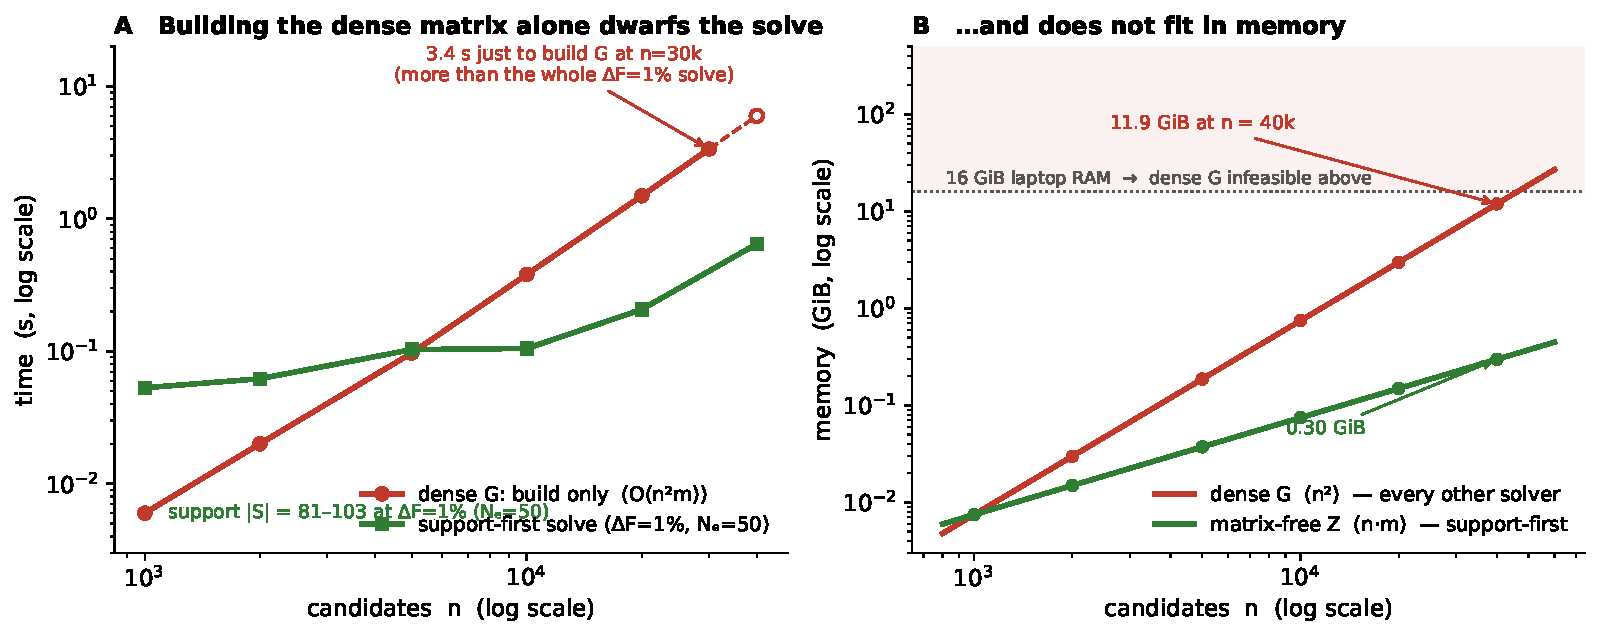
\includegraphics[width=\linewidth]{fig_scaling.pdf}
\caption{Passage à l'échelle sans matrice contre $\bG$ dense à un point de fonctionnement de sélection ($\Delta F=1~\%$, $N_e=50$). \textbf{(A)} La seule construction de la $\bG$ dense ($O(n^2 m)$) dépasse la résolution support-first entière, dont le support reste borné (${\sim}80$--103) et le temps autour de 0,3~s quand $n$ croît jusqu'à 40000. \textbf{(B)} Mémoire : la $\bG$ dense atteint 11,9~Gio à $n=40000$ contre 0,30~Gio pour la $\bZ$ sans matrice. Les courbes de construction et de mémoire sont indépendantes du point de fonctionnement.}
\label{fig:scaling}
\end{figure}

\subsection{Comportement du support}

L'avantage repose sur le support, dont la taille est fixée par le point de fonctionnement --- le taux de consanguinité cible $\Delta F$, soit le nombre effectif de parents $N_e\approx1/(2\Delta F)$ --- et non par une constante universelle ; aussi l'ancrons-nous aux bornes qu'utilisent réellement les programmes de sélection plutôt qu'à une borne favorable. Les programmes tournent à $\Delta F$ d'environ 0,5 à 2~\% ; le plancher FAO est $N_e\ge50$, soit $\Delta F\le1~\%$. À ces bornes, le support sur les panels ici est de quelques dizaines à deux cents, non de quelques unités : sur la souris, 47 candidats sur 1814 à $\Delta F=2~\%$, 89 à 1~\% et 182 à 0,5~\% (une borne lâche, à l'inverse, l'effondre à deux, et $N_e\approx10$). Deux comportements sont à distinguer. \emph{Le long} de la frontière, le support croît à mesure qu'on pousse la diversité --- sur la souris, 47/89/182 à $\Delta F=2/1/0,5~\%$, montant à ${\sim}1163$ à l'approche de la coancestrie minimale. \emph{À travers} la taille de population, à point de fonctionnement fixé, il reste borné : sur des panels structurés (AlphaSimR) à $\Delta F=1~\%$, le support se maintient autour de 90 quand $n$ croît de 1000 à 40000, tandis que la $\bG$ dense croît jusqu'à 11,9~Gio. Une borne \emph{absolue} fixée, à l'inverse, ne fait paraître le support plat quand $n$ croît que parce que la coancestrie minimale atteignable décroît en ${\sim}1/n$ et relâche ainsi la contrainte --- d'où notre choix de fixer le point de fonctionnement, non la borne. La question de savoir si le support est borné indépendamment du point de fonctionnement reste ouverte ; la génétique fournit la moitié « croissance » ($\Delta F\propto\sum c_i^2$), et la Discussion reprend le reste. La Figure~\ref{fig:frontier} montre les deux sur les panels réels : le support le long de $\Delta F$ (A) et le temps de résolution sans matrice (B), ce dernier ordonné par le nombre de marqueurs.

\begin{figure}[ht]
\centering
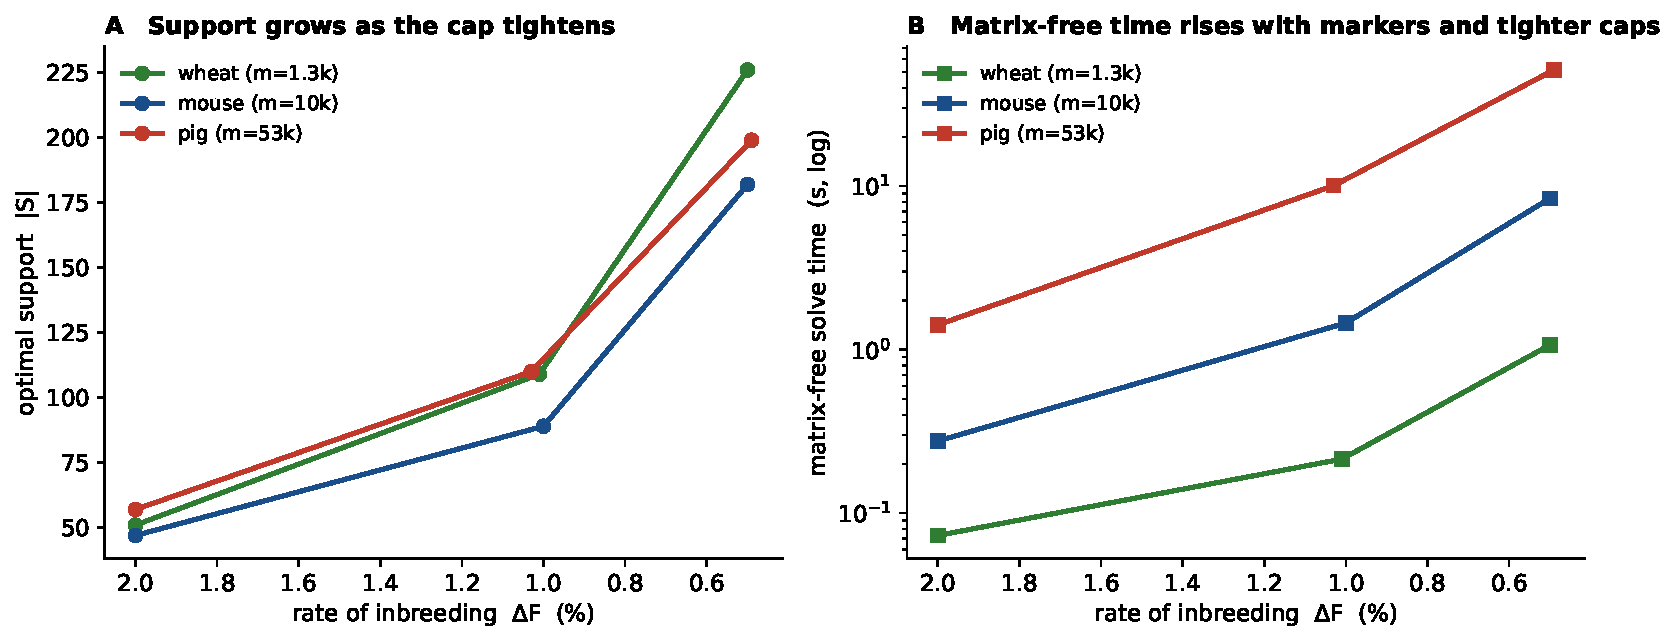
\includegraphics[width=\linewidth]{fig_frontier.pdf}
\caption{La frontière du point de fonctionnement sur les trois panels réels. \textbf{(A)} Le support optimal croît quand la borne de coancestrie se resserre (plus petit $\Delta F$, plus grand $N_e\approx1/(2\Delta F)$). \textbf{(B)} Le temps de résolution sans matrice croît avec la borne et, à $\Delta F$ fixé, avec le nombre de marqueurs $m$ --- porc (53k SNP) au-dessus de souris (10k) au-dessus de blé (1,3k) --- le coût $O(nm)$ par itération rendu visible.}
\label{fig:frontier}
\end{figure}

\subsection{Validation multi-générations}

Les résultats mono-génération établissent l'exactitude et le coût ; la question de sélection est de savoir si support-first appliqué en récurrent se comporte comme doit le faire la sélection à contribution optimale au fil des générations. Nous avons simulé 12 générations de sélection récurrente sur des populations AlphaSimR (120 fondateurs coalescents, un caractère additif, 3 répétitions), chaque génération appelant le binding R livré pour résoudre l'OCS à $\Delta F=1~\%$ ($N_e=50$) sur les génotypes courants et croiser proportionnellement aux contributions rendues, face à la sélection par troncature (les 25 meilleurs de chaque sexe par valeur génétique vraie) comme référence indifférente à la diversité. Support-first conserve nettement plus de diversité --- l'hétérozygotie observée tombe à 0,246 à la génération 12 contre 0,221 pour la troncature (toutes deux depuis 0,290), une perte ${\sim}40~\%$ plus lente --- tout en \emph{soutenant} le gain : il égale la troncature tôt et la dépasse légèrement tard (11,9 contre 11,6 à la génération 12, Figure~\ref{fig:multigen}), car maintenir bas le taux de consanguinité préserve la variance génétique dont se nourrit la réponse à long terme. C'est le cas d'école de l'OCS, reproduit avec support-first pilotant chaque génération.

\begin{figure}[ht]
\centering
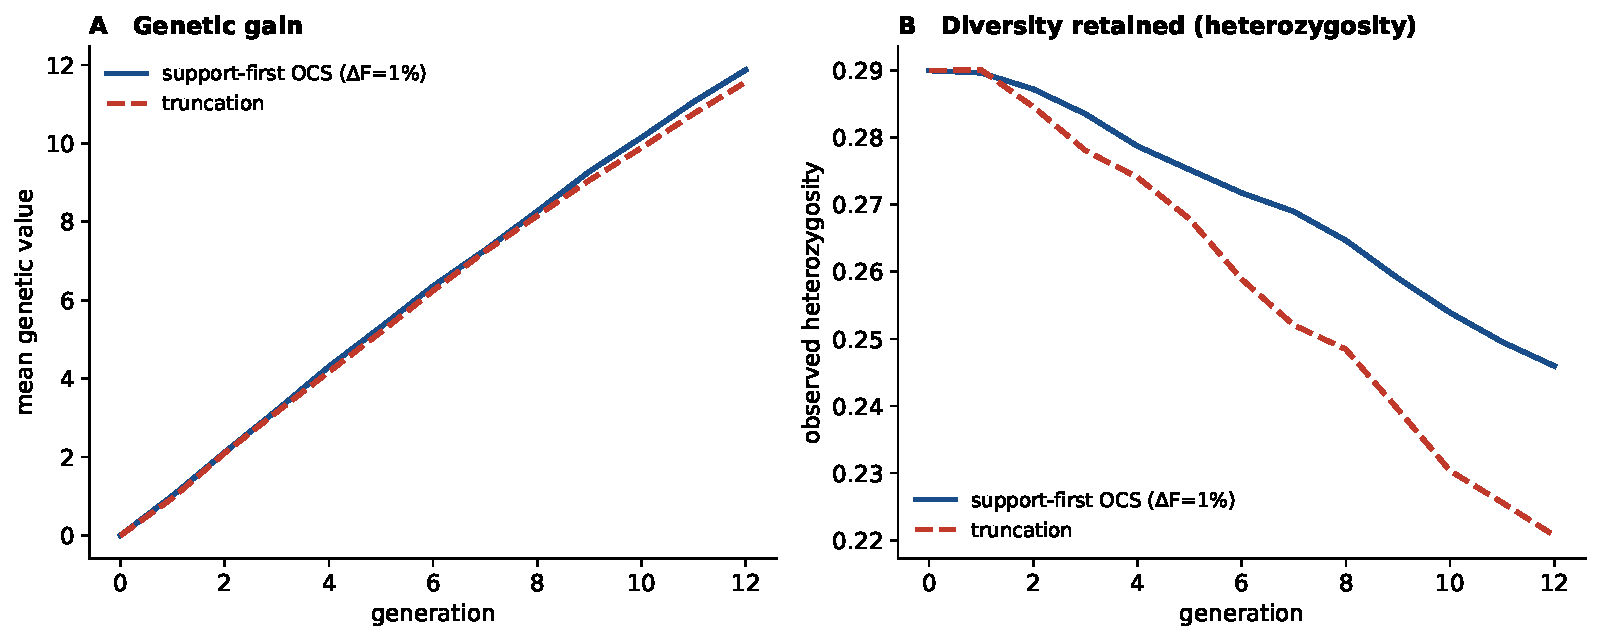
\includegraphics[width=\linewidth]{fig_multigen.pdf}
\caption{Douze générations de sélection récurrente sur populations AlphaSimR (3 répétitions) : support-first OCS à $\Delta F=1~\%$ contre troncature. \textbf{(A)} Gain génétique --- OCS égale la troncature et la dépasse tard. \textbf{(B)} Hétérozygotie observée --- OCS la conserve nettement mieux (0,246 contre 0,221 à la génération 12), la variance préservée soutenant le gain en (A).}
\label{fig:multigen}
\end{figure}

\section{Discussion}

Support-first rend la sélection à contribution optimale exacte peu coûteuse à l'échelle génomique, en deux sens distincts. Recevant la matrice de parenté, son ensemble actif atteint le même optimum que la résolution à point intérieur d'optiSel un à deux ordres de grandeur plus vite aux bornes pertinentes pour la sélection (12 à 132$\times$ ici), en exploitant la parcimonie du support à une évaluation en $O(n^2)$. Et en formant les produits de parenté sans matrice, il ne stocke jamais la matrice dense, restant ainsi exécutable précisément là où cette matrice devient infaisable --- le régime à grand nombre de candidats qui motive l'OCS génomique. La voie sans matrice est l'élément habilitant, non une accélération universelle : son coût de $O(nm)$ par itération la rend plus lente que la réutilisation d'une $\bG$ précalculée quand les marqueurs dépassent largement les candidats, comme sur le porc. La méthode étant exacte et déterministe --- un ensemble actif certifié Karush--Kuhn--Tucker plutôt qu'une recherche stochastique --- sa sortie est reproductible jusqu'au dernier chiffre, contrairement aux outils heuristiques de sélection d'accouplements auxquels elle est comparée.

Les ingrédients de la méthode sont individuellement classiques, et nous n'en revendiquons que la synthèse. Le suivi par ensemble actif d'un petit ensemble de travail descend de l'algorithme de la ligne critique pour la sélection moyenne--variance long-only ; la forme fermée par support est un résultat de valeur propre contrainte ; le produit sans matrice est standard en prédiction génomique. La contribution est leur combinaison, spécialisée à l'OCS : une génération de colonnes par coût réduit qui fait croître un support restreint vers une unique borne de coancestrie, avec le produit de parenté évalué sans matrice de sorte que le coût suit le support et le nombre de marqueurs plutôt que la matrice $n\times n$. Située face aux travaux antérieurs les plus proches, ce n'est ni la parcimonie de la matrice de pedigree d'un solveur OCS à point intérieur, ni les résolutions denses sur toute la population des outils de référence. Deux comparaisons plus proches que nous n'avons pas exécutées, et que nous signalons plutôt que d'écarter. Gencont2 (Dagnachew \& Meuwissen 2016) est un Newton--Raphson sur les conditions lagrangiennes à $O(n^2)$ par itération --- le même coût par itération que notre pricing ---, donc à coût égal c'est le test juste de savoir si un ensemble actif croissant converge en moins d'itérations qu'un Newton sur l'ensemble complet ; sa distribution est liée aux relations généalogiques et nous ne l'avons pas réimplémenté sur une $\bG$ génomique, ce qui est le benchmark le plus informatif encore ouvert. Le solveur ADMM/JuMP de Waldmann (2025) forme $\bG$ explicitement et heurterait le mur mémoire à grand $n$, mais est parfaitement benchmarkable sur les petits panels ici ; nous laissons les deux à des travaux futurs plutôt que d'invoquer une incomparabilité.

Plusieurs limites bornent ces résultats. Premièrement, le critère de sélection est une valeur génétique estimée réelle sur les panels porcins et un phénotype enregistré en tenant lieu sur le blé et la souris. Sur le sous-panel porcin sexué, nous avons de plus utilisé une vraie GEBV, ajustée par GBLUP sur les phénotypes et la matrice de parenté de ce panel, sans que le résultat change : les conclusions ne dépendent donc pas de la valeur génétique retenue comme critère. Sur le blé et la souris, en revanche, le critère demeure un phénotype, et les vecteurs de contributions restent dans tous les cas illustratifs plutôt que des recommandations de sélection. Deuxièmement, un sexe réellement enregistré est disponible pour le panel souris et pour le sous-panel porcin sexué --- la seule instance combinant une vraie valeur génétique et un sexe réel, et donc ce qui se rapproche le plus ici d'un problème OCS opérationnel ---, tandis que le blé et le panel porcin complet reçoivent une répartition équilibrée arbitraire. Ce sous-panel porte sa propre restriction : le sexe se déduit du pedigree précisément pour les animaux devenus parents, c'est donc un sous-ensemble post-sélection des candidats et non un échantillon aléatoire de ceux-ci. Troisièmement, le Tableau~\ref{tab:optisel} sépare deux choses que l'énoncé de vitesse confondait. Recevant $\bG$ dense, l'ensemble actif atteint l'optimum d'optiSel 12 à 132$\times$ plus vite aux bornes pertinentes pour la sélection, évaluant en $O(n^2)$ indépendamment du nombre de marqueurs --- le résultat algorithmique. Le solveur sans matrice, ne formant aucun $\bG$, paie au contraire $O(nm)$ par itération : il n'est plus rapide que jusqu'à une densité de marqueurs modérée et est \emph{plus lent} qu'optiSel sur le porc à 52k SNP (0,3$\times$), où réutiliser une $\bG$ formée une fois bat la re-dérivation de la parenté depuis $\bZ$ à ce petit $n$ (le \emph{binding} est lui-même sans copie, c'est donc le solve, non une copie). Ce 0,3$\times$ reflète un flux dense-$f64$ naïf de $\bZ$, non une limite intrinsèque : stocker $\bZ$ à deux bits par génotype et paralléliser le produit rendent la même résolution sans matrice 3,1$\times$ plus rapide aux dimensions du porc (optimum identique à la précision machine), réduisant l'écart à la voie avec $\bG$ fournie. Les deux coïncident dans le mécanisme --- le même ensemble actif --- et ne diffèrent que par la matérialisation de $\bG$. La voie sans matrice est l'élément habilitant en mémoire et à grand $n$ ; l'accélération algorithmique sur les solveurs à point intérieur est le petit ensemble actif. Quatrièmement, le caractère borné du support optimal est, dans cet article, une observation empirique sur un balayage synthétique et les panels réels, et pas encore un théorème, et la voie est plus subtile qu'un comptage de contraintes. Sans ridge ($\varepsilon=0$, $\bG=\bZ\bZ\tp/s$ de rang $r$), un argument propre le borne : l'optimum maximise un lagrangien qui ne dépend de $\bc$ qu'à travers $(\bZ\tp\bc,\ \bb\tp\bc)$, de sorte que la tranche optimale $\{\bA\bc=\bd,\ \bc\ge0,\ \bZ\tp\bc=\bZ\tp\bc^\star,\ \bb\tp\bc=\bb\tp\bc^\star\}$ est un polytope LP dont les sommets portent $\le q+r+1$ composantes non nulles --- une borne de point extrême / Carathéodory, indépendante de $n$, sur exactement le sommet que renvoie un solveur à ensemble actif comme support-first (les solveurs à point intérieur et ADMM renvoient au contraire des points intérieurs non parcimonieux qu'ils seuillent a posteriori). Cette borne est toutefois vide dans le régime génomique qu'elle vise : avec $m>n$ marqueurs, $r=\mathrm{rang}(\bZ\bZ\tp)=n-1$, de sorte que $q+r+1$ dépasse $n$ et la borne se lit $|S|\le n$ sur chaque panel réel ici --- elle ne mord que si $m<n$. Le support empirique est une petite fraction de $n$, de sorte que l'énoncé utile du caractère borné est empirique, non ce théorème. Le ridge opératoire $\varepsilon>0$ rend de plus $\bG$ de plein rang, et nous constatons numériquement que le support réalisé n'est alors pas gouverné par rang($\bG_0$) : il reste une petite fraction de $n$ (dizaines à quelques centaines selon la borne) et stable en $n$ à borne fixée, mais ne se réduit pas à une unique quantité spectrale propre --- le rang effectif est suggestif mais, sur un balayage de spectres, n'est pas un prédicteur fiable --- de sorte qu'une borne serrée pour le problème ridgé reste ouverte. La génétique rend compte de la croissance : $\Delta F\propto\sum c_i^2$ (Wray \& Thompson 1990 ; Woolliams \& Bijma 2000) avec $N_e\approx1/(2\Delta F)$, de sorte que resserrer la borne étale les contributions et fait croître le support, comme observé. Nous développons cette caractérisation dans des travaux ultérieurs. Enfin, le solveur gère une unique contrainte quadratique de parenté, des plafonds de contribution par candidat ($0\le\bc\le\bu$) et les égalités de sexe, mais pas encore plusieurs contraintes quadratiques à la fois --- matrices de parenté multiples, limites de coancestrie spécifiques à des groupes --- ni l'allocation entière des accouplements que fournit AlphaMate ; il renvoie des contributions continues.

Une limite du travail mérite d'être énoncée clairement, car elle décide de ce qui est éprouvé et de ce qui ne l'est pas. Ce travail a été mené sans convention d'accès institutionnelle : chaque panel utilisé est donc téléchargeable par n'importe quel lecteur et chaque chiffre du présent article est régénérable à partir de sources publiques --- un gain délibéré de reproductibilité, et un plafond réel sur l'échelle. Les plus grandes populations réelles en sélection animale se trouvent dans les bases d'évaluation nationales, qui comptent des centaines de milliers d'animaux génotypés et dont l'accès est contrôlé ; la plus grande ressource bovine de séquences librement disponible compte quelques milliers d'individus, moins que le panel porcin employé ici. Les résultats de passage à l'échelle à $n=10^4$--$4\times10^4$ sont donc synthétiques par nécessité et non par préférence. Ce qu'ils établissent --- que la matrice de parenté dense devient infaisable avant le solveur --- est une propriété de cette matrice et ne dépend pas du caractère réel des génotypes. Ce qu'ils n'établissent pas, c'est la méthode s'exécutant au sein d'une évaluation en production à cette échelle, et aucun jeu de données public ne peut l'établir. Cette comparaison exige un organisme de sélection ou un centre d'évaluation national, et nous l'accueillerions volontiers.

Chaque limite indique une extension. Le c\oe ur en forme fermée par support admet déjà plus d'une contrainte d'égalité via la même élimination $\mathbf{P}=\bA\bG^{-1}\bA\tp$ ; des plafonds quadratiques actifs supplémentaires transforment la recherche de racine scalaire en un petit système de faible degré plutôt qu'ils n'en changent la structure, de sorte que des contraintes de parenté multiples sont à portée. Une couche d'arrondi ou de séparation et évaluation (branch-and-bound) au-dessus de l'optimum continu ajouterait l'allocation des accouplements tout en gardant la relaxation exacte comme borne serrée --- combinant l'exactitude de support-first avec le plan discret que les heuristiques visent directement. Le basculement sans matrice en $m$ versus $n$ mérite une caractérisation explicite, tout comme la borne de support elle-même. Et la méthode devrait être validée sur des populations un ordre de grandeur plus grandes, où l'écart mémoire passe de visible à décisif ; la question du critère est désormais close sur une instance, une GEBV ajustée par GBLUP sur le sous-panel porcin sexué ne changeant rien.

Support-first fait une chose --- la sélection à contribution optimale exacte, à contrainte unique, continue --- à une échelle et une vitesse qui mettent l'OCS génomique à portée d'un ordinateur portable et d'un script reproductible. Cette affirmation étroite et vérifiée, et les extensions ouvertes qu'elle invite, constituent la contribution.

\section*{Disponibilité des données et du code}

Le solveur support-first ainsi que tous les scripts de comparaison et de reproduction sont disponibles à \url{https://github.com/Adelagric/ocs-rs} (licence MIT) et archivés sur Zenodo (\url{https://doi.org/10.5281/zenodo.20746987}). Chaque tableau et figure est régénéré par \texttt{research/repro/repro.sh}, dont les étapes portent le nom du tableau ou de la figure qu'elles produisent ; une étape dont la chaîne d'outils ou le jeu de données manque est ignorée avec un message. Deux exceptions sont délibérées : le point $n=10000$ de Clarabel (Tableau~\ref{tab:clarabel}) ne s'exécute que sous \texttt{REPRO\_FULL=1} (Clarabel y demande ${\sim}26$ minutes), et la comparaison AlphaMate se lance manuellement depuis un binaire émulé. Les panels de marqueurs sont publics : les panels blé et souris sont fournis avec le paquet R BGLR (Pérez \& de los Campos 2014) ; le panel de porc PIC est le jeu de données commun de Cleveland, Hickey \& Forni (2012) (DOI 10.1534/g3.111.001453).

\section*{Références}
\sloppy

\subsection*{Méthodes et outils OCS}
\begin{enumerate}
\item \textbf{Meuwissen, T.H.E. (1997).} Maximizing the response of selection with a predefined rate of inbreeding. \emph{Journal of Animal Science} 75(4):934--940. DOI 10.2527/1997.754934x.
\item \textbf{Dagnachew, B.S. \& Meuwissen, T.H.E. (2016).} A fast Newton--Raphson based iterative algorithm for large scale optimal contribution selection. \emph{Genetics Selection Evolution} 48(1):70. DOI 10.1186/s12711-016-0249-2.
\item \textbf{Pong-Wong, R. \& Woolliams, J.A. (2007).} Optimisation of contribution of candidate parents to maximise genetic gain and restricting inbreeding using semidefinite programming. \emph{Genetics Selection Evolution} 39(1):3--25. DOI 10.1186/1297-9686-39-1-3.
\item \textbf{Wellmann, R. (2019).} Optimum contribution selection for animal breeding and conservation: the R package optiSel. \emph{BMC Bioinformatics} 20(1):25. DOI 10.1186/s12859-018-2450-5.
\item \textbf{Gorjanc, G. \& Hickey, J.M. (2018).} AlphaMate: a program for optimizing selection, maintenance of diversity and mate allocation in breeding programs. \emph{Bioinformatics} 34(19):3408--3411. DOI 10.1093/bioinformatics/bty375.
\item \textbf{Waldmann, P. (2025).} Genomic optimum contribution selection and mate allocation using JuMP. \emph{Bioinformatics Advances} 5(1):vbaf259. DOI 10.1093/bioadv/vbaf259.
\item \textbf{Yamashita, M., Mullin, T.J. \& Safarina, S. (2018).} An efficient second-order cone programming approach for optimal selection in tree breeding. \emph{Optimization Letters} 12(7):1683--1697. DOI 10.1007/s11590-018-1229-y ; arXiv:1506.04487. --- Exploite la parcimonie de l'\emph{inverse du pedigree}, pas le support de la solution.
\end{enumerate}

\subsection*{Parenté génomique et produits sans matrice}
\begin{enumerate}\setcounter{enumi}{7}
\item \textbf{VanRaden, P.M. (2008).} Efficient methods to compute genomic predictions. \emph{Journal of Dairy Science} 91(11):4414--4423. DOI 10.3168/jds.2007-0980.
\item \textbf{Legarra, A. \& Misztal, I. (2008).} Technical note: Computing strategies in genome-wide selection. \emph{Journal of Dairy Science} 91(1):360--366. DOI 10.3168/jds.2007-0403.
\end{enumerate}

\subsection*{Filiation ensemble actif et forme fermée (antériorité reconnue)}
\begin{enumerate}\setcounter{enumi}{9}
\item \textbf{Markowitz, H. (1956).} The optimization of a quadratic function subject to linear constraints. \emph{Naval Research Logistics Quarterly} 3(1--2):111--133. DOI 10.1002/nav.3800030110. --- L'algorithme de la ligne critique.
\item \textbf{Gander, W., Golub, G.H. \& von Matt, U. (1989).} A constrained eigenvalue problem. \emph{Linear Algebra and its Applications} 114--115:815--839. DOI 10.1016/0024-3795(89)90494-1. --- La forme fermée par support (équation séculaire).
\end{enumerate}

\subsection*{Logiciels et données}
\begin{enumerate}\setcounter{enumi}{11}
\item \textbf{Goulart, P.J. \& Chen, Y. (2024).} Clarabel: an interior-point solver for conic programs with quadratic objectives. arXiv:2405.12762. (Version évaluée par les pairs : \emph{Mathematical Programming Computation}, 2026, DOI 10.1007/s12532-026-00320-7.) --- Utilisé uniquement comme oracle de contre-vérification indépendant.
\item \textbf{Quiñones, S.} faer: a linear-algebra library for the Rust programming language. Logiciel, version 0.24.0 (épinglée dans \texttt{Cargo.toml}) ; \url{https://github.com/sarah-quinones/faer-rs}. (Soumission JOSS en cours d'examen ; pas de DOI publié à ce jour.)
\item \textbf{Pérez, P. \& de los Campos, G. (2014).} Genome-wide regression and prediction with the BGLR statistical package. \emph{Genetics} 198(2):483--495. DOI 10.1534/genetics.114.164442. --- Source des panels blé (CIMMYT) et souris.
\item \textbf{Cleveland, M.A., Hickey, J.M. \& Forni, S. (2012).} A common dataset for genomic analysis of livestock populations. \emph{G3: Genes|Genomes|Genetics} 2(4):429--435. DOI 10.1534/g3.111.001453. --- Le panel de porc PIC.
\end{enumerate}

\section*{Annexe : la taille du support --- un encadrement}
Le coût de support-first suit la taille du support $|S|$ ; on l'encadre (preuves complètes, identité KKT de liaison et carte empirique dans la note compagne \texttt{research/support\_bound\_sketch.md}, scripts reproductibles \texttt{research/bound\_*.py}).

\textbf{Théorème 1 (borne sans ridge).} \emph{Pour $\varepsilon = 0$ ($\bG = \bZ\bZ\tp/s$ de rang $r \le m$), l'OCS atteint son optimum en un vecteur de contributions de support $|S| \le q + r + 1$, indépendant de $n$} ($q \in \{1,2\}$ lignes de budget). À $\varepsilon = 0$ le lagrangien ne dépend de $\bc$ qu'à travers $(\bZ\tp\bc,\ \bb\tp\bc) \in \mathbb{R}^{r+1}$ ; fixer ces quantités linéarise la face optimale en un polytope LP dont les sommets ont $\le q + r + 1$ composantes non nulles --- le sommet que renvoie un solveur à ensemble actif. (Carathéodory / Barvinok--Pataki sur la face linéarisée, pas sur la frontière courbe de l'ellipsoïde, où $\bG$ définie positive rend tout point extrême.)

\textbf{Théorème 2 (aucune borne universelle avec le ridge).} \emph{Pour $\bG = \bZ\bZ\tp/s + \varepsilon\mathbf{I}$ ($\varepsilon > 0$), aucune borne $f(q, r)$ indépendante de $n$ ne tient --- le support peut valoir $n$.} Témoin : $\bG = \varepsilon\mathbf{I}$ (aucun marqueur, tous non apparentés) réduit le cap de parenté à $\varepsilon\lVert\bc\rVert^2 \le k$, où $\lVert\bc\rVert^2$ est le proxy du taux de consanguinité ; juste au-dessus du minimum uniforme la boule réalisable force le support plein (vérifié à $n = 300$). C'est la limite sans structure.

Entre les deux, le support réalisé est fixé par la géométrie conjointe de (spectre, $\bb$, cap $k$) : petit et stable en $n$ précisément quand le spectre décroît et que $\bb$ évite les directions propres dominantes --- sur les panels réels ici, $|S|$ va de dizaines à quelques centaines selon la borne (47/89/182 sur la souris à $\Delta F=2/1/0,5\%$) --- mais sans loi scalaire prédictive unique. Le borner sous cette structure réaliste est le problème ouvert. Développement complet : \texttt{research/support\_bound\_sketch.md} (et \texttt{support\_bound\_fr.tex}).

\end{document}
